%! Author = spruhs
%! Date = 25.02.25

% Preamble
\documentclass[11pt]{article}

% Packages
\usepackage[utf8]{inputenc}
\usepackage[T1]{fontenc}
\usepackage[ngerman]{babel}
\usepackage{graphicx}
\usepackage{tcolorbox}
\usepackage{tocloft}
\usepackage{appendix}
\usepackage{csquotes}
\usepackage[
    backend=biber,
    style=alphabetic,
]{biblatex}
\usepackage{color}
\usepackage{listings}
\usepackage{xcolor}
\usepackage{hyperref}
\usepackage[a4paper, left=3cm, right=3cm]{geometry}
\addbibresource{literaturverzeichnis.bib}


% Farben für Syntax-Highlighting definieren
\definecolor{codegreen}{rgb}{0,0.6,0}
\definecolor{codegray}{rgb}{0.5,0.5,0.5}
\definecolor{codepurple}{rgb}{0.58,0,0.82}
\definecolor{backcolour}{rgb}{0.95,0.95,0.92}

% Kotlin-Sprache für listings konfigurieren
\lstdefinelanguage{Kotlin}{
    morekeywords={fun, class, object, val, var, when, if, else, for, while, return, import, package, is, as, null, true, false},
    sensitive=true,
    morecomment=[l]{//},
    morecomment=[s]{/*}{*/},
    morestring=[b]",
}

% Java-Sprache für listings konfigurieren (Java ist bereits vordefiniert, aber hier ein Beispiel für Anpassungen)
\lstdefinelanguage{Java}{
    morekeywords={public, private, protected, class, static, void, if, else, while, for, return, import, package, new},
    sensitive=true,
    morecomment=[l]{//},
    morecomment=[s]{/*}{*/},
    morestring=[b]",
}

\lstset{
    backgroundcolor=\color{backcolour},
    commentstyle=\color{codegreen},
    keywordstyle=\color{codepurple},
    numberstyle=\tiny\color{codegray},
    stringstyle=\color{red},
    basicstyle=\ttfamily\footnotesize,
    breakatwhitespace=false,
    breaklines=true,
    captionpos=b,
    keepspaces=true,
    numbers=left,
    numbersep=5pt,
    showspaces=false,
    showstringspaces=false,
    showtabs=false,
    tabsize=2
}

% Document
\begin{document}

    \begin{titlepage}
        \centering
        {\scshape\LARGE Seminar 1908 Moderne Programmiertechniken und -Methoden -Sommer 2025 \par}
        \vspace{1cm}
        {\huge\bfseries Kotlin statt Java\par}
        \vspace{1.5cm}
        {\scshape\Large Fabian Spruhs\par}
        {\scshape fabian@spruhs.com\par}
        \vspace{2cm}
        {\Large\itshape Studiengang Bachelor Informatik\par}
        \vspace{2cm}


        {\large \today\par}
    \end{titlepage}

    \tableofcontents
    \newpage

    \section{Einleitung}
    Java ist den meisten Entwicklern ein Begriff.
    Es ist eine weit verbreitete Programmiersprache, die seit ihrer Einführung im Jahr 1995 eine zentrale Rolle in der Softwareentwicklung spielt~\cite[49]{insel}.
    Kotlin ist eine relativ neue Programmiersprache, die 2011 von JetBrains veröffentlicht wurde.
    Sie wurde mit dem Ziel entwickelt, eine moderne und verbesserte Alternative zu Java zu schaffen~\cite[19]{kotlin-handbuch}.\\
    \\
    In diesem Text werden die Unterschiede zwischen Java und Kotlin untersucht.
    Es wird untersucht, inwieweit Kotlin eine geeignete Alternative zu Java darstellt und welche Vorteile Kotlin gegenüber Java bietet.
    Zunächst werden beide Programmiersprachen kurz vorgestellt.
    Anschließend wird auf die Interoperabilität zwischen Java und Kotlin eingegangen.
    Dabei soll gezeigt werden, inwieweit sich Java und Kotlin in einem Projekt kombinieren lassen, bzw. wie bestehende Java-Projekte mit Kotlin weitergeführt werden können.\\
    \\
    Danach werden die unterschiedlichen Features der Sprachen untersucht.
    Zuerst gibt es eine kurze Übersicht über die Features die Kotlin von Java unterscheiden.
    Danach werden die wichtigsten Features genauer erläutert, also die Features die einen tatsächlichen Mehrwert bieten.
    Dabei wird hauptsächlich auf die Unterschiede zwischen Java und Kotlin eingegangen.
    Wie diese Features konkret genutzt werden kann nur am Rande besprochen werden, da dies den Umfang des Textes sprengen würde.\\
    \\
    Zum Schluss gibt es ein Fazit und eine kurze Zusammenfassung der Ergebnisse.
    Die Codebeispiele in diesem Text können auf GitHub unter \url{github.com/FSpruhs/kotlin-statt-java} gefunden werden und können alle, zu Testzwecken, selber ausgeführt werden.\\
    \\
    \section{Kurzvorstellung Java}

    \subsection{Übersicht}
    \begin{itemize}
        \item \textbf{Erscheinungsjahr:} 1995
        \item \textbf{Entwickler:} Sun Microsystems
        \item \textbf{Entwickler ab 2009:} Oracle Corporation
        \item \textbf{Programmier paradigmen:} objektorientiert
        \item \textbf{Aktuelle LTS version:} 21
    \end{itemize}

    \subsection{Technischer Hintergrund}
    Java ist eine Programmiersprache, die von Sun Microsystems entwickelt und im Jahr 1995 veröffentlicht wurde.
    Sie zeichnet sich durch ihre Plattformunabhängigkeit, hohe Robustheit und vielseitigen Einsatzmöglichkeiten aus,wodurch sie insbesondere in der Industrie und im Unternehmensumfeld eine zentrale Rolle spielt.\\
    \\
    Ein wesentliches Merkmal von Java ist die Art der Code-Ausführung.
    Anstatt direkt in Maschinencode übersetzt zu werden, wird der Quellcode zunächst in Bytecode kompiliert.
    Dieser Bytecode wird anschließend von der Java Virtual Machine (JVM) interpretiert und ausgeführt.
    Durch dieses Konzept ist Java nicht an eine spezifische Prozessorarchitektur oder ein bestimmtes Betriebssystem gebunden, was eine hohe Portabilität gewährleistet.
    Diese Plattformunabhängigkeit stellt einen bedeutenden Vorteil dar, den viele andere Programmiersprachen im Laufe der Zeit übernommen haben.\\
    \\
    Neben der Plattformunabhängigkeit bietet die JVM zahlreiche zusätzliche
    Funktionen, die zur Stabilität und Sicherheit von Java-Anwendungen beitragen.
    Dazu gehören unter anderem eine automatische Speicherverwaltung
    durch den Garbage Collector, eine starke Typisierung zur Minimierung
    von Laufzeitfehlern sowie eine integrierte Unterstützung für Multithreading,
    die eine effiziente nebenläufige Verarbeitung ermöglicht. \cite[51 - 54]{insel}\\
    \\
    Java basiert konsequent auf dem objektorientierten Programmierparadigma, das die Strukturierung von Software in Klassen und Objekte ermöglicht. \\
    \\
    \subsection{Verbreitung}
    Der TIOBE-Index misst monatlich die Popularität und Verbreitung von Programmiersprachen~\cite{tiobe}.
    Laut diesem Index zählt Java zu den am weitesten verbreiteten Programmiersprachen weltweit.
    Wie in Abbildung~\ref{fig:entwicklung-tiobe} ersichtlich, befand sich Java über fast zwei Jahrzehnte hinweg
    kontinuierlich unter den Top 3 der relevantesten Programmiersprachen.\\
    \\
    In den letzten Jahren hat die Popularität von Java zwar leicht nachgelassen, dennoch bleibt die Sprache weiterhin
    von großer Bedeutung.
    Auch im Februar 2025 belegte Java den dritten Platz im TIOBE-Index (siehe Abbildung~\ref{fig:tiobe-java-2025}).\\
    \\
    Java ist die Basis zahlreicher Anwendungen und wird in vielfältigen Bereichen eingesetzt.
    Darüber hinaus verfügt Java über eine umfangreiche Ökosystemlandschaft mit einer Vielzahl an Bibliotheken, Paketen,Frameworks und Fachliteratur.\\
    \\
    Die weltweite Java-Community ist äußerst aktiv und umfasst eine große Anzahl an erfahrenen Entwicklern, die kontinuierlich zum Wissenstransfer und zur Weiterentwicklung der Sprache beitragen.
    Ein Beispiel für die Größe dieser Infrastruktur ist das Maven-Repository, das über 2.800 Repositories mit mehr als 52 Millionen Java-Paketen enthält~\cite{maven}.\\
    \\
    Diese etablierte und breit aufgestellte Infrastruktur stellt einen weiteren entscheidenden Vorteil von Java dar und
    trägt zu seiner anhaltenden Relevanz in der Softwareentwicklung bei.\\

    \section{Kurzvorstellung kotlin}

    \subsection{Übersicht}
    \begin{itemize}
        \item \textbf{Erscheinungsjahr:} 2011
        \item \textbf{Entwickler:} Jetbrains
        \item \textbf{Programmier paradigmen:} objektorientiert, funktional
        \item \textbf{Aktuelle LTS version:} 2.1.0
    \end{itemize}

    \subsection{Technischer Hintergrund}
    Kotlin wurde 2011 von der Firma JetBrains veröffentlicht.
    Ziel der Entwicklung war es, eine verbesserte Alternative zu Java zu schaffen(vgl~\cite[19]{kotlin-handbuch}).
    Schon an der Namensgebung kann man die nähe zu Java erkennen.
    Der Name Java bezieht sich auf eine Indonesische Insel.
    Der Namensgeber von Kotlin ist eine russische Insel vor St. Petersburg.\\
    \\
    Obwohl Java nur etwa 15 Jahre älter als Kotlin ist, stellt dies in der schnelllebigen Welt der Softwareentwicklung eine erhebliche Zeitspanne dar.
    In vielerlei Hinsicht wirkt Java inzwischen veraltet.
    Die Syntax ist vergleichsweise umständlich, und einige moderne Sprachfeatures, die in anderen Programmiersprachen standardmäßig verfügbar sind, fehlen in Java oder
    müssen umständlich über externe Tools nachgerüstet werden.
    Zudem setzt Java ausschließlich auf das objektorientierte Paradigma,
    während moderne Programmiersprachen häufig eine Kombination aus objektorientierter und funktionaler Programmierung unterstützen.\\
    \\
    Bei der Entwicklung von Kotlin hat JetBrains bewusst aus den Designfehlern von Java gelernt.
    Gleichzeitig wurden essenzielle Eigenschaften, die zur Popularität von Java beigetragen haben, beibehalten.\\
    \\
    Kotlin-Code wird ebenfalls in Bytecode kompiliert und kann auf der Java Virtual Machine (JVM) ausgeführt werden.
    Dies bietet den großen Vorteil, dass Kotlin-Programme überall dort lauffähig sind, wo auch Java-Code ausgeführt werden kann.
    Zudem kann Kotlin auf sämtliche vorhandenen Java-Bibliotheken zugreifen und diese nutzen, wodurch nahezu das gesamte Java-Ökosystem zur Verfügung steht.
    Die Interoperabilität zwischen Kotlin und Java geht sogar noch weiter.
    Beide Sprachen lassen sich nahtlos in einem Projekt kombinieren.
    Dadurch können auch bestehende Java-Anwendungen schrittweise mit Kotlin weiterentwickelt werden~\cite[19-20]{kotlin-handbuch}.\\
    \\
    \subsection{Verbreitung}
    Nach dem TIOBE index befindet sich Kotlin im März 2025 nur auf Platz 19 der relevantesten Sprachen, siehe Abbildung~\ref{fig:tiobe-kotlin-2025}.
    Es gibt aber auch gute Nachrichten für Kotlin im Bezug auf die Verbreitung und relevanz.
    Kotlin wurde von Google zu der bevorzugten Sprache für die Android Entwicklung erklärt~\cite{tn3-google}.\\
    \\
    \section{Interoperabilität zwischen Java und Kotlin}

    \subsection{Kotlin in Java integrieren}
    Kotlin und Java lassen sich nahtlos in einem Projekt kombinieren, was zahlreiche Vorteile mit sich bringt.
    Zum einen können in Kotlin geschriebene Klassen und Funktionen problemlos in Java verwendet werden und umgekehrt.
    Zum anderen ermöglicht diese Interoperabilität, bestehende Java-Projekte schrittweise mit Kotlin weiterzuentwickeln oder nach und nach auf Kotlin umzustellen, ohne den vorhandenen Code sofort ersetzen zu müssen.
    Dies ist besonders für Unternehmen mit großen Java-Codebasen relevant, die nicht abrupt auf Kotlin wechseln können~\cite[20]{kotlin-handbuch}.\\
    \\
    Im folgenden Beispiel werden verschiedene Möglichkeiten vorgestellt, wie Kotlin-Code in einer Java-Umgebung ausgeführt werden kann.
    Die zugehörige \texttt{.java}-Datei enthält eine Java-Klasse mit einer \texttt{main}-Methode.
    In dieser Datei wird Kotlin-Code aus einer \texttt{.kt}-Datei importiert und ausgeführt, da Kotlin-Quellcode stets
    in Dateien mit der Endung \texttt{.kt} gespeichert wird.\\
    \\

    \begin{lstlisting}[language=Kotlin, caption={KotlinGreeter.kt}]

class ClassGreeter {
    fun greet() {
        println("Hello from kotlin class method!")
    }
}

class StaticGreeter {
    companion object {

        @JvmStatic
        fun greet() {
            println("Hello from kotlin static method!")
        }
    }
}
object SingletonGreeter {
    fun greet() {
        println("Hello from kotlin singleton method!")
    }
}
    \end{lstlisting}

    \begin{lstlisting}[language=Java, caption={Main.java}]
import main.java.com.spruhs.ClassGreeter;
import main.java.com.spruhs.SingletonGreeter;
import main.java.com.spruhs.StaticGreeter;

public static void main(String[] args) {
    ClassGreeter classGreeter = new ClassGreeter();
    classGreeter.greet();

    StaticGreeter.greet();

    SingletonGreeter.INSTANCE.greet();
}
    \end{lstlisting}

    \begin{tcolorbox}[colback=black!5!white, colframe=black, title=Ausgabe]
        Hello from kotlin class method!\\
        Hello from kotlin static method!\\
        Hello from kotlin singleton method!
    \end{tcolorbox}
    
    \subsection{Java in Kotlin integrieren}
    Auch die umgekehrte Richtung ist problemlos möglich.
    Java-Code lässt sich ohne Weiteres in Kotlin verwenden.
    Dies bietet insbesondere den Vorteil, dass bestehende Java-Bibliotheken und -Frameworks weiterhin genutzt werden können.
    Dies spielt für viele Kotlin-Projekte eine entscheidende Rolle, insbesondere wenn auf etablierte Java-Ökosysteme wie Spring oder Hibernate zurückgegriffen wird.\\
    \\
    Im folgenden Beispiel werden zwei verschiedene Arten gezeigt, wie Java-Klassen in Kotlin eingebunden werden können.
    Einmal über eine Instanzmethode und einmal über eine statische Methode.\\
    \\
    Die Integration von Java in Kotlin ist besonders einfach, da Kotlin die Java-Klassen so behandelt, als wären sie eigene Kotlin-Klassen.
    Statische Methoden und Felder werden in Kotlin über den Klassennamen aufgerufen, Instanzmethoden funktionieren analog wie in Kotlin selbst.
    Damit bietet Kotlin ein hohes Maß an Interoperabilität mit Java, was den Umstieg oder die parallele Nutzung beider Sprachen deutlich vereinfacht.\\
    \\

    \begin{lstlisting}[language=Java, caption={JavaClassMethodGreeter.java}]

public class JavaClassMethodGreeter {
    public void greet() {
        System.out.println("Hello from java class method!");
    }
}
    \end{lstlisting}

    \begin{lstlisting}[language=Java, caption={JavaStaticGreeter.java}]

public class JavaStaticGreeter {
    public static void greet() {
        System.out.println("Hello from java static method!");
    }
}

    \end{lstlisting}

    \begin{lstlisting}[language=Kotlin, caption={Main.kt}]

fun main() {
    val javaClassMethodGreeter = JavaClassMethodGreeter()
    javaClassMethodGreeter.greet()

    JavaStaticGreeter.greet()
}
    \end{lstlisting}

    \begin{tcolorbox}[colback=black!5!white, colframe=black, title=Ausgabe]
        Hello from java class method!\\
        Hello from java static method!\\
    \end{tcolorbox}

    \section{Features}

    \subsection{Kurzübersicht}

    In der folgenden Tabelle~\ref{tab:kotlin-java-features} werden zentrale Sprachfeatures aufgeführt, durch die sich Kotlin von Java unterscheidet.
    Anschließend werden einige der wichtigsten Unterschiede genauer erläutert.\\
    \\
    Bei den Features, die Java besitzt, die aber in Kotlin nicht mehr vorhanden sind, lässt sich zwischen vollständig entfallenen Funktionen und solchen unterscheiden, die durch alternative Konzepte ersetzt wurden.\\
    \\
    Ein klassisches Beispiel hierfür sind \texttt{static} Members.
    Kotlin kennt das \texttt{static}-Schlüsselwort nicht.
    Stattdessen bietet Kotlin das Konzept der \texttt{Companion Objects}, um Klassenfunktionen und Klasseneigenschaften zu definieren, die unabhängig von einer konkreten Instanz verfügbar sein sollen.\\
    \\
    Auch das in Java etablierte Konzept der Wildcards (wie \texttt{? extends T} oder \texttt{? super T}) zur Variabilität in generischen Typen wird in Kotlin nicht verwendet.
    An dessen Stelle treten in Kotlin zwei modernere Mechanismen: die Declaration-Site Variance (z.B. \texttt{out T} oder \texttt{in T}) und \texttt{Type Projections}, die eine bessere Lesbarkeit und Typensicherheit ermöglichen.\\
    \\
    Der aus Java bekannte Ternary-Operator (\texttt{condition ? trueExpr : falseExpr}) entfällt in Kotlin vollständig, da \texttt{if}-Anweisungen dort als Ausdrücke gestaltet sind und somit selbst einen Wert zurückgeben können.
    Dadurch lässt sich die gleiche Funktionalität deutlich eleganter realisieren.\\
    \\
    Das Pattern-Matching wird in Kotlin durch die Smart-Casts ersetzt.\\
    \\
    Die mit Java 14 eingeführten \texttt{Records}, die als einfache, immutable Datencontainer dienen, wurden in Kotlin durch die \texttt{data class} ersetzt.
    Diese bieten ähnliche Vorteile, wie automatische Implementierungen von \texttt{equals()}, \texttt{hashCode()} und \texttt{toString()}.\\
    \\
    Checked Exceptions, ein markantes Merkmal der Java-Fehlerbehandlung, existieren in Kotlin nicht mehr.
    Diese Entscheidung wurde bewusst getroffen, da checked exceptions oft als hinderlich für die Lesbarkeit und Wartbarkeit des Codes empfunden werden.
    Fehlerbehandlung in Kotlin erfolgt stattdessen durch unchecked exceptions oder alternative Ansätze wie das Result-Typ-Pattern.
    Hierzu bietet Kotlin den \texttt{Result}-Typ, der eine elegante Möglichkeit zur Handhabung von Erfolgen und Fehlern in einer Funktion bietet.\\
    \\
    Ein weiterer Unterschied liegt in der Sichtbarkeit von Klassen und Mitgliedern.
    Während Java das Schlüsselwort \texttt{package-private} (also ohne Sichtbarkeitsmodifikator) kennt, wurde diese Möglichkeit in Kotlin entfernt.
    In Kotlin gibt es stattdessen die Schlüsselwörter \texttt{public}, \texttt{internal}, \texttt{protected} und \texttt{private}.\\
    \\
    Schließlich ist auch der Umgang mit primitiven Datentypen unterschiedlich: Java unterscheidet streng zwischen primitiven Typen (z.B. int, boolean) und ihren Wrapper-Klassen (Integer, Boolean).
    In Kotlin gibt es diese Trennung nicht auf Sprachebene.
    Hier sind alle Typen Klassen.
    Allerdings sorgt der Kotlin-Compiler dafür, dass im Bytecode bei Bedarf trotzdem die entsprechenden Java-Primitives verwendet werden, um keine Performanceeinbußen zu verursachen~\cite{doc-comparison}.

    \begin{table}[h!]
        \centering
        \begin{tabular}{|c|c|}
            \hline
            \textbf{Kotlin-Features, die Java nicht hat} & \textbf{Java-Features, die Kotlin nicht hat} \\
            \hline
            \hline
            Lambda expressions & Checked Exceptions \\
            \hline
            Inline functions & Primitive types \\
            \hline
            Extension functions & Wildcard-types \\
            \hline
            Null-safety & Ternary-Operator \\
            \hline
            Default properties & Records \\
            \hline
            Smart casts & Static members \\
            \hline
            Primary constructors & Pattern Matching \\
            \hline
            First-class delegation & package-private visibility modifier \\
            \hline
            Declaration-site variance and Type projections &  \\
            \hline
            Singletons &  \\
            \hline
            Range expressions &  \\
            \hline
            Operator overloading &  \\
            \hline
            Companion objects &  \\
            \hline
            Data classes &  \\
            \hline
            Coroutines &  \\
            \hline
            Top-level functions &  \\
            \hline
            Default arguments &  \\
            \hline
            Named parameters &  \\
            \hline
            Infix functions &  \\
            \hline
            Expect and actual declarations &  \\
            \hline
            Explicit API Mode and better control of API surface &  \\
            \hline
        \end{tabular}
        \caption{Vergleich Kotlin und Java Features}
        \label{tab:kotlin-java-features}
    \end{table}

    \subsection{Null-safety}
    Tony Hoare war 1965 an der Einführung der ersten Null-Referenz in der objektorientierten Sprache ALGOL W beteiligt.
    Im Jahr 2009 bezeichnete er dies rückblickend als den „Milliarden-Dollar-Fehler“~\cite{billion-dollar-mistake}.
    Auch in Java wurde dieser Fehler durch die Einführung von \texttt{null} als Referenzwert übernommen.
    In Java können alle Referenztypen, mit Ausnahme der primitiven Datentypen, den Wert \texttt{null} annehmen.\\
    \\
    Dies führt in der Praxis häufig zu sogenannten \texttt{NullPointerException}, ein weit verbreiteter Laufzeitfehler in Java-Anwendungen.
    Um diese zu vermeiden, müsste man theoretisch jede Referenz vor dem Zugriff auf \texttt{null} prüfen.
    In der Realität wird das jedoch selten konsequent umgesetzt.
    Dies würde auch zu umfangreichem Boilerplate-Code führt, der die Lesbarkeit und Wartbarkeit des Codes stark beeinträchtigen kann.\\
    \\
    Kotlin hat aus diesem Konzeptionsfehler gelernt und verfolgt einen strikt null-sicheren Ansatz.
    In Kotlin sind Referenzen standardmäßig \texttt{non-nullable}.
    Ein Wert kann nur dann \texttt{null} sein, wenn der entsprechende Typ explizit als \texttt{nullable} deklariert wurde.
    Die geschieht durch Anhängen eines Fragezeichens (\texttt{?}) an den Typnamen.
    Der Kotlin-Compiler erzwingt daraufhin eine explizite Überprüfung, wodurch potenzielle \texttt{NullPointerException} bereits zur Compile-Zeit erkannt und vermieden werden können.\\
    \\
    Dieses Sprachfeature trägt erheblich zur Robustheit und Stabilität von Kotlin-Programmen bei, da viele Fehlerquellen bereits zur Entwicklungszeit erkannt werden.
    Darüber hinaus vereinfacht es das Debugging und beschleunigt die Fehlersuche deutlich.
    In Listing~\ref{lst:kotlin-null-safety} wird dieses Prinzip anhand eines einfachen Beispiels verdeutlicht.
    Zwei Variablen des Typs \texttt{String} werden deklariert.
    Eine davon ist \texttt{nullable}, die andere nicht.
    Während der \texttt{nullable} Variablen problemlos \texttt{null} zugewiesen werden kann, führt der gleiche Versuch bei der \texttt{non-nullable} Variablen zu einem Compilerfehler.\\
    \\
    Zusätzlich stellt Kotlin elegante Sprachmittel zur Verfügung, um mit null-Werten umzugehen:

    \begin{itemize}

        \item
            Der Safe-Call-Operator (\texttt{?.}) ermöglicht den Zugriff auf Eigenschaften oder Methoden eines Objekts, ohne zuvor explizit auf null prüfen zu müssen.
            Ist die Referenz \texttt{null}, wird \texttt{null} zurückgegeben, anstatt eine Exception auszulösen.
        \item
            Der Elvis-Operator (\texttt{?:}) erlaubt es, für den Fall eines \texttt{null}-Werts einen Default-Wert zu definieren.
    \end{itemize}

    Diese Mechanismen werden in Listing~\ref{lst:kotlin-user-null-safety} anhand der \texttt{data class KotlinUser} demonstriert.
    Die Funktion \texttt{getUserName} nimmt ein \texttt{nullabel} Objekt entgegen und gibt entweder den enthaltenen Namen oder, falls das Objekt \texttt{null} ist, einen Fallback-Wert zurück.\\
    \\
    Im Vergleich dazu zeigt Listing~\ref{lst:java-user-null-safety} das gleiche Beispiel in Java.
    Dabei wird deutlich, wie viel mehr Boilerplate-Code erforderlich ist, um das gleiche Sicherheitsniveau zu erreichen.\\
    \\

    \begin{lstlisting}[language=Kotlin, caption={KotlinNullSafety.kt}, label={lst:kotlin-null-safety}]

fun testNullSafety() {
    var nullableVariable: String?
    var nonNullableVariable: String

    nullableVariable = null // Kein Compiler Fehler
    nonNullableVariable = null // Compiler Fehler
}
    \end{lstlisting}

    \begin{lstlisting}[language=Kotlin, caption={KotlinUser.kt}, label={lst:kotlin-user-null-safety}]

fun getUserName(user: KotlinUser?): String {
    return user?.name ?: "Unbekannter Benutzer"
}

data class KotlinUser(val name: String)

fun main() {
    val user1: KotlinUser = KotlinUser("Fabian")
    val user2: KotlinUser? = null

    println(getUserName(user1)) // Ausgabe: Fabian
    println(getUserName(user2)) // Ausgabe: Unbekannter Benutzer
}
    \end{lstlisting}

    \begin{lstlisting}[language=Java, caption={NullHandlingExample.java}, label={lst:java-user-null-safety}]

class JavaUser {
    private String name;

    public JavaUser(String name) {
        this.name = name;
    }

    public String getName() {
        return name;
    }
}

public class NullHandlingExample {
    public static String getUserName(JavaUser user) {
        return (user != null && user.getName() != null)
                ? user.getName() : "Unbekannter Benutzer";
    }

    public static void main(String[] args) {
        JavaUser user1 = new JavaUser("Fabian");
        JavaUser user2 = null;

        System.out.println(getUserName(user1)); // Ausgabe: Fabian
        System.out.println(getUserName(user2)); // Ausgabe: Unbekannter Benutzer
    }
}
    \end{lstlisting}

    \subsection{Funktionale Programierung}

    Die funktionale Programmierung hat in den letzten Jahren zunehmend an Bedeutung gewonnen.
    Ein wesentlicher Grund dafür liegt in der stagnierenden Entwicklung der CPU-Geschwindigkeit.
    Während in früheren Jahren Leistungssteigerungen hauptsächlich durch höhere Taktfrequenzen erzielt wurden, liegt der Fokus heute verstärkt auf Mehrkernprozessoren.
    Daraus ergibt sich die Notwendigkeit, Programme parallel auszuführen, um die vorhandenen Ressourcen effizient zu nutzen.\\
    \\
    Die funktionale Programmierung eignet sich besonders gut für Parallelisierungskonzepte, da sie auf Zustandslosigkeit und Nebenwirkungsfreiheit basiert.
    Diese Eigenschaften vereinfachen die Ausführung von Code und machen sie zugleich sicherer~\cite[129]{kotlin-patterns}.\\
    \\
    Kotlin wurde von Beginn an mit dem Ziel entwickelt, eine moderne Programmiersprache bereitzustellen, die sowohl objektorientierte als auch funktionale Paradigmen unterstützt.
    Im Gegensatz dazu wurde Java ursprünglich als rein objektorientierte Sprache konzipiert und hat erst mit Version 8 funktionale Sprachmerkmale wie Lambda-Ausdrücke und Streams eingeführt.\\
    \\
    Im Folgenden werden einige der wichtigsten funktionalen Konzepte von Kotlin vorgestellt und mit entsprechenden Merkmalen in Java verglichen.
    Ziel ist es, die Unterschiede sowie die jeweiligen Stärken beider Sprachen im funktionalen Kontext zu verdeutlichen.

    \subsubsection{Higher-Order-Functions}
    Kotlin unterstützt sogenannte Higher-Order Functions.
    Das sind Funktionen, die andere Funktionen als Parameter entgegennehmen oder selbst Funktionen zurückgeben können.
    Funktionen sind in Kotlin sogenannte \textit{First-Class Citizens}, was bedeutet, dass sie wie andere Datentypen behandelt werden können, z.B. indem man sie Variablen zuweist oder als Rückgabewerte verwendet.\\
    \\
    In Java hingegen können Funktionen nicht direkt übergeben werden, da Java ursprünglich keine funktionalen Konzepte vorsah.
    Stattdessen wurde Funktionalität in Methoden gekapselt, die Teil eines Objekts sind.
    Erst mit der Einführung von Lambda-Ausdrücken in Kombination mit functional Interfaces sowie Methoden- und Konstruktorreferenzen in Java 8 wurde eine kompakte Syntax eingeführt, mit der sich Funktionalität auch ohne explizite Klassendefinition umsetzen lässt~\cite[820]{insel}.\\
    \\
    In den folgenden beiden Codebeispielen ist jeweils eine Funktion dargestellt, die zwei Zahlen sowie eine weitere Funktion als Parameter entgegennimmt.
    Diese übergebene Funktion nimmt ebenfalls zwei Zahlen entgegen und gibt eine einzelne Zahl zurück.\\
    \\
    Listing~\ref{lst:kotlin-higher-order-function} zeigt die Kotlin-Variante, während Listing~\ref{lst:java-higher-order-function} die Java-Implementierung darstellt.

    An der Kotlin-Implementierung wird deutlich, dass keine zusätzliche Klasse erforderlich ist.
    Die Funktion kann direkt als Parameter übergeben werden.
    In Java hingegen ist die Übergabe einer Funktion nur über ein funktionales Interface möglich.
    In diesem Fall \texttt{BiFunction}.
    Dieses muss zusätzlich importiert werden.\\
    \\
    Kotlin bietet in diesem Zusammenhang eine deutlich elegantere und direktere Möglichkeit, funktionale Konzepte zu nutzen, da es keine zusätzlichen Konstrukte wie funktionale Interfaces benötigt.\\
    \\

    \begin{lstlisting}[language=Kotlin, caption={HigherOrderKotlin.kt}, label={lst:kotlin-higher-order-function}]

fun operateOnNumbers(a: Int, b: Int, operation: (Int, Int) -> Int): Int {
    return operation(a, b)
}

fun main() {
    val sum = operateOnNumbers(5, 3) { x, y -> x + y }
    println(sum) // Ausgabe 8
}
    \end{lstlisting}

    \begin{lstlisting}[language=Java, caption={HigherOrderJava.java}, label={lst:java-higher-order-function}]

import java.util.function.BiFunction;

public class HigherOrderJava {

    public static int operateOnNumbers(int a, int b, BiFunction<Integer, Integer, Integer> operation) {
        return operation.apply(a, b);
    }

    public static void main(String[] args) {
        int sum = operateOnNumbers(5, 3, (x, y) -> x + y);
        System.out.println(sum); // Ausgabe 8
    }
}
    \end{lstlisting}

    \subsubsection{Inline Functions}
    Kotlin unterstützt sogenannte Inline Functions, mit denen sich der Overhead von Funktionsaufrufen reduzieren lässt.
    Dies ist besonders nützlich in Verbindung mit Higher-Order Functions, da es die Performance verbessert und den generierten Bytecode optimiert.\\
    \\
    Ein vergleichbares Feature in Java sind Lambda-Ausdrücke.
    Diese bieten jedoch nicht den gleichen Grad an Optimierung wie die Inline-Funktionen in Kotlin.
    Bei einer Inline-Funktion wird der Funktionscode direkt an der Aufrufstelle in den Bytecode eingefügt, anstatt zur Laufzeit aufgerufen zu werden.
    Dadurch wird der Overhead vermieden, der bei normalen Funktionsaufrufen entsteht.\\
    \\
    Listing~\ref{lst:kotlin-inline-function} zeigt eine Inline-Funktion in Kotlin.
    Die Funktion \texttt{transformString} nimmt einen \texttt{String} sowie eine Funktion entgegen, die einen \texttt{String} als Parameter akzeptiert und ebenfalls einen \texttt{String} zurückgibt.
    Die übergebene Funktion wird auf den Eingabestring angewendet.
    In diesem Fall wird er in Großbuchstaben umgewandelt.
    Dabei wird bei dem Aufruf der Funktion die übergebene Funktion inline in den Code eingefügt.
    Dies wird durch das Schlüsselwort \texttt{inline} erreicht~\cite{kotlin-inline}.\\
    \\

    \begin{lstlisting}[language=Kotlin, caption={InlineFunction.java}, label={lst:kotlin-inline-function}]

inline fun transformString(
    input: String,
    transform: (String) -> String
): String {
    return transform(input)
}

fun main() {
    val result = transformString("Hello, World!") { it.uppercase() }
    println(result) // Ausgabe: HELLO, WORLD!
}
    \end{lstlisting}

    \subsection{Threads und Coroutines}

    \subsubsection{Laufzeitverhalten}

    In modernen Anwendungen, insbesondere in solchen mit hoher Benutzerinteraktion oder paralleler Datenverarbeitung, spielt effiziente Nebenläufigkeit eine zentrale Rolle.
    Während sich funktionale Programmierung gut eignet, um nebenläufige Logik deklarativ und fehlerarm zu beschreiben, reicht dies allein nicht aus, um die tatsächliche Ausführung effizient zu gestalten.\\
    \\
    In Java werden Threads verwendet, um parallele Ausführung zu ermöglichen.
    Ein Java-Thread ist eine 1:1-Abbildung auf einen Betriebssystem-Thread~\cite[940]{insel}.
    Das bedeutet, dass jeder Java-Thread direkt mit einem nativen Thread des Betriebssystems verknüpft ist.
    Jedem Thread wird dabei ein eigener Stack und Speicherbereich zugewiesen.
    Da Threads relativ schwergewichtig sind und mit nicht unerheblichem Overhead verbunden sind, ist die Anzahl parallel laufender Threads begrenzt.
    Eine zu hohe Thread-Anzahl kann schnell zu einem Mangel an Systemressourcen führen.\\
    \\
    Ein gängiger Lösungsansatz in Java sind sogenannte Thread-Pools.
    Dabei handelt es sich um eine feste Anzahl von Threads, die wiederverwendet werden, um Aufgaben auszuführen.
    Wenn ein Thread im Pool blockiert, kann kein weiterer hinzugefügt werden, bis ein anderer Thread wieder freigegeben wird.
    Dies kann zu einer suboptimalen Auslastung der Systemressourcen führen.\\
    \\
    Kotlin bietet mit Coroutines eine leichtgewichtigere Alternative.
    Coroutines ermöglichen eine effizientere und zugleich einfachere Umsetzung von paralleler und asynchroner Programmierung.
    Sie sind nicht an einen bestimmten System-Thread gebunden und können flexibel zwischen Threads wechseln.
    Die Verwaltung der Coroutines übernimmt der Kotlin-Compiler in Verbindung mit dem Dispatcher, der auch den Overhead von Kontextwechseln reduziert.
    Selbst bei einer blockierenden Coroutine bleibt der zugrunde liegende Thread frei und kann andere Coroutines verarbeiten.
    So lässt sich eine deutlich bessere Ausnutzung der verfügbaren Ressourcen erzielen~\cite[194]{kotlin-patterns}.\\
    \\
    In Listing~\ref{lst:kotlin-coroutine} wird eine Schleife mit 10.000 Iterationen implementiert.
    In jeder Iteration wird ein Zähler erhöht, eine kurze Pause eingelegt und der Zähler erneut erhöht.
    Diese Schleife wird sowohl mit Coroutines als auch mit Threads (mittels Thread-Pool) umgesetzt.
    Beide Varianten werden nach spätestens 20 Sekunden beendet oder sobald alle Iterationen abgeschlossen sind.\\
    \\
    Die Ausführungszeiten sind in Tabelle~\ref{tab:coroutine-thread-pool} dargestellt.
    Hier zeigt sich deutlich der Effizienzvorteil von Coroutines.
    Sie sind deutlich schneller als Threads, da sie ressourcenschonender arbeiten und nicht direkt an System-Threads gebunden sind.
    Mehrere Coroutines können gleichzeitig auf einem Thread laufen, da blockierende Operationen den Thread nicht blockieren.
    Der Dispatcher übernimmt das Scheduling und sorgt dafür, dass nur aktive Coroutines weiter ausgeführt werden.\\
    \\
    Umso mehr Threads genutzt werden, desto schneller wird die Ausführungszeit.
    Zwischen 2.500 und 5.000 Threads ist die Ausführungszeit fast gleich.
    Dafür ist aber der Speicherverbrauch deutlich höher.
    Ab 10.000 Threads, also genau der Anzahl an Iterationen, kommt es sogar zu einem \texttt{OutOfMemoryError}.\\
    \\
    Dieses Beispiel verdeutlicht, dass Coroutines eine deutlich leichtgewichtigere und skalierbarere Alternative zu klassischen Threads darstellen.
    Die Messungen wurden auf einem Ubuntu 24.04 System mit 8~GB RAM und einem AMD Ryzen 5 4500U (6 Kerne) durchgeführt.
    Das Ergebnis ist auch in Abbildung~\ref{fig:coroutines-threads} zu sehen.\\
    \\

    \begin{lstlisting}[language=Kotlin, caption={Coroutines.kt}, label={lst:kotlin-coroutine}]

import kotlinx.coroutines.*
import java.util.concurrent.CountDownLatch
import java.util.concurrent.Executors
import java.util.concurrent.TimeUnit
import java.util.concurrent.atomic.AtomicInteger

fun coroutineTest() {
    val latch = CountDownLatch(10_000)
    val counter = AtomicInteger()

    val start = System.currentTimeMillis()
    runBlocking {
        for (i in 1..10_000) {
            launch {
                counter.incrementAndGet()
                delay(100)
                counter.incrementAndGet()
                latch.countDown()
            }
        }
    }

    latch.await(20, TimeUnit.SECONDS)

    println("Execution time: ${System.currentTimeMillis() - start} ms, Counter: ${counter.get()/2}")
}

fun threadTest(threadPoolSize: Int) {
    val counter = AtomicInteger()

    val pool = Executors.newFixedThreadPool(threadPoolSize)
    val start = System.currentTimeMillis()
    for (i in 1..10_000) {
        pool.submit {
            counter.incrementAndGet()
            Thread.sleep(100)
            counter.incrementAndGet()
        }
    }

    pool.shutdown()
    pool.awaitTermination(20, TimeUnit.SECONDS)

    println("ThreadPoolSize: $threadPoolSize, execution time: ${System.currentTimeMillis() - start} ms, Counter: ${counter.get()/2}")
}

fun main() {
    coroutineTest()
    listOf(1, 10, 50, 100, 1_000, 2_500, 5_000, 10_000).forEach {
        threadTest(it)
    }
}
    \end{lstlisting}

    \begin{table}[h!]
        \centering
        \begin{tabular}{|c|c|c|c|}
            \hline
             & \textbf{Ausführungszeit} & \textbf{Counter}\\
            \hline
            Coroutines & 410 ms & 10.000   \\
            \hline
            Thread-Pool 1 & 20.011 ms  & 199  \\
            \hline
            Thread-Pool 10 & 20.007 ms  & 1.995  \\
            \hline
            Thread-Pool 50 & 20.008 ms  & 9.975  \\
            \hline
            Thread-Pool 100 & 10.015 ms  & 10.000  \\
            \hline
            Thread-Pool 1.000 & 1.048 ms  & 10.000  \\
            \hline
            Thread-Pool 2.500 & 574 ms  & 10.000  \\
            \hline
            Thread-Pool 5.000 & 562 ms  & 10.000  \\
            \hline
            Thread-Pool 10.000 & OutOfMemoryError  &   \\
            \hline
        \end{tabular}
        \caption{Ausführungszeiten von Coroutines und Threads}
        \label{tab:coroutine-thread-pool}
    \end{table}
    
    \subsubsection{Channels}
    Ein zentrales Merkmal der Kotlin-Coroutines ist die Unterstützung für Channels, die eine einfache Möglichkeit bieten, Daten zwischen Coroutines zu übermitteln.
    Channels ermöglichen es, dass zwei oder mehr Coroutines effizient und nebenläufig miteinander kommunizieren können.
    Dabei müssen keine Synchronisationsmechanismen wie Locks oder Shared Mutable State verwendet werden.
    Dies vereinfacht die Entwicklung nebenläufiger Anwendungen erheblich und trägt zur Fehlerminimierung bei~\cite[208]{kotlin-patterns}.\\
    \\
    Channels lassen sich in Kotlin wie Queues verwenden.
    Eine Coroutine sendet Daten in den Channel, eine andere empfängt sie.\\
    \\
    In Listing~\ref{lst:kotlin-channels} wird ein Channel<Int> erstellt, in den eine Coroutine Zahlen von 1 bis 5 sendet.
    Eine zweite Coroutine empfängt diese Zahlen und gibt sie aus.
    Die Nutzung von channel.close() signalisiert, dass keine weiteren Werte mehr folgen, sodass die empfangende Coroutine korrekt beendet werden kann.\\
    \\
    In Listing~\ref{lst:java-channels} wird das gleiche Beispiel in Java umgesetzt.
    Hier gibt es jedoch keine native Unterstützung für Channels, wie Kotlin sie bietet.
    Um ein ähnliches Verhalten zu erreichen, kann eine BlockingQueue verwendet werden, wobei jedoch auf die Synchronisation und die korrekte Beendigung selbst geachtet werden muss.
    In der Java-Version müssen eigene Threads erzeugt werden, und zur Signalisierung des Endes dient ein spezieller Wert (-1), da es keine eingebaute close()-Funktion wie bei Kotlin-Channels gibt.\\
    \\

    \begin{lstlisting}[language=Kotlin, caption={Channels.kt}, label={lst:kotlin-channels}]

import kotlinx.coroutines.*
import kotlinx.coroutines.channels.Channel

fun channelsExample() = runBlocking {
    val channel = Channel<Int>()

    launch {
        for (x in 1..5) {
            println("Send $x")
            channel.send(x)
        }
        channel.close()
    }

    launch {
        for (y in channel) {
            println("Receive $y")
        }
    }
}

fun main() {
    channelsExample()
}
    \end{lstlisting}

    \begin{lstlisting}[language=Java, caption={JavaChannels.java}, label={lst:java-channels}]

import java.util.concurrent.*;

public class JavaChannels {
    public static void main(String[] args) throws InterruptedException {
        BlockingQueue<Integer> queue = new LinkedBlockingQueue<>();

        Thread producer = new Thread(() -> {
            try {
                for (int i = 1; i <= 5; i++) {
                    System.out.println("Sende " + i);
                    queue.put(i);
                }
                queue.put(-1);
            } catch (InterruptedException e) {
                Thread.currentThread().interrupt();
            }
        });

        Thread consumer = new Thread(() -> {
            try {
                while (true) {
                    int value = queue.take();
                    if (value == -1) break;
                    System.out.println("Receive " + value);
                }
            } catch (InterruptedException e) {
                Thread.currentThread().interrupt();
            }
        });

        producer.start();
        consumer.start();
        producer.join();
        consumer.join();
    }
}
    \end{lstlisting}

    \subsection{Syntax verbesserungen}
    Kotlin bietet eine Vielzahl von Sprachfeatures, die darauf abzielen, den Code kompakter, lesbarer und weniger fehleranfällig zu machen.
    Viele dieser Konzepte lassen sich grundsätzlich auch in Java umsetzen, erfordern dort jedoch deutlich mehr Boilerplate-Code und führen zu weniger übersichtlichem Quelltext.
    Auch wenn man einige dieser Features als „Syntax-Sugar“ bezeichnen könnte, ergibt sich durch deren Zusammenspiel ein spürbarer Mehrwert in Bezug auf Produktivität und Wartbarkeit.
    Im Folgenden werden die wichtigsten dieser Sprachfeatures vorgestellt und ihre Vorteile gegenüber Java erläutert.

    \subsubsection{Extension Functions}
    Kotlin bietet die Möglichkeit, bestehende Klassen um neue Funktionen zu erweitern, ohne deren Quellcode zu verändern oder von ihnen erben zu müssen.
    Diese sogenannten Extension Functions können wie reguläre Methoden auf Instanzen aufgerufen werden.\\
    \\
    Besonders praktisch ist, dass sich mit Extension Functions nicht nur eigene Klassen erweitern lassen, sondern auch Klassen aus externen Bibliotheken.
    Dadurch können fehlende Funktionalitäten bequem nachgerüstet werden, ohne bestehende Strukturen zu verändern.\\
    \\
    In Listing~\ref{lst:kotlin-extension-function} wird eine Extension Function \texttt{double} für die Klasse \texttt{String} implementiert.
    Die Definition erfolgt durch Voranstellen des Klassennamens vor den Funktionsnamen, getrennt durch einen Punkt.
    Innerhalb der Funktion kann mit dem Schlüsselwort \texttt{this} auf die aktuelle Instanz zugegriffen werden.
    Die Methode verdoppelt den Inhalt des Strings und gibt diesen zurück.\\
    \\
    In der \texttt{main}-Methode wird die Funktion zweimal aufgerufen.
    Besonders in Zeile 8 zeigt sich die Eleganz der Kotlin-Syntax.
    Die Erweiterung lässt sich direkt auf dem String-Objekt aufrufen, als wäre sie eine native Methode der \texttt{String}-Klasse.\\
    \\
    Auch in Java ist es prinzipiell möglich, bestehende Klassen zu erweitern.
    Die lässt sich beispielsweise durch das Decorator-Pattern oder Vererbung realisieren.
    Diese Lösungen sind jedoch deutlich aufwändiger, führen zu mehr Boilerplate-Code und sind in der Praxis oft weniger flexibel~\cite{kotlin-extensions}.\\
    \\

    \begin{lstlisting}[language=Kotlin, caption={ExtensionFunction.kt}, label={lst:kotlin-extension-function}]

fun String.double(): String {
    return "$this $this"
}

fun main() {
    val name = "Hello World!".double()
    println(name.double()) // Output: Hello World! Hello World! Hello World! Hello World!
}
    \end{lstlisting}

    \subsubsection{Named Parameters, Properties und Primary Constructor}
    Named Parameters und Properties sind zwei Sprachfeatures von Kotlin, die besonders in Kombination ihre Stärke entfalten.
    Sie ermöglichen eine flexible und zugleich lesbare Art der Objektkonstruktion, die in Java meist nur mit zusätzlichem Boilerplate-Code erreichbar ist.\\
    \\
    \textbf{Named Parameters} erlauben es, Funktions- oder Konstruktorparameter explizit mit Namen anzugeben.
    Dies verbessert die Lesbarkeit und erlaubt es, Parameter in beliebiger Reihenfolge zu übergeben oder nur jene anzugeben, die tatsächlich notwendig sind.\\
    \\
    \textbf{Properties} ermöglichen es, Klassenattribute direkt im Konstruktor zu deklarieren.
    Gemeinsam mit dem Konzept des \textbf{Primary Constructors}, der in Kotlin direkt in der Klassendeklaration definiert wird, lassen sich Klassen deutlich kompakter und intuitiver schreiben.\\
    \\
    In Listing~\ref{lst:kotlin-builder-pattern} wird am Beispiel des Builder Patterns gezeigt, wie diese Features zusammenwirken.
    Das Builder Pattern ist ein klassisches Entwurfsmuster aus der „Gang of Four“-Sammlung, das häufig zur Konstruktion komplexer Objekte mit vielen optionalen Parametern verwendet wird~\cite[139]{gang-of-four}.\\
    \\
    In der Klasse \texttt{User} werden die Attribute \texttt{firstName}, \texttt{lastName}, \texttt{titles} und \texttt{age} im Primary Constructor definiert.
    Alle mit Default-Werten.
    Dadurch wird der Builder überflüssig, da sich Objekte flexibel und übersichtlich direkt über den Konstruktor erstellen lassen.
    In der \texttt{main}-Methode wird ein Objekt mit allen Attributen und ein weiteres nur mit \texttt{firstName} und \texttt{lastName} erstellt~\cite[46]{kotlin-patterns}.\\
    \\
    Zum Vergleich zeigt Listing~\ref{lst:java-builder-pattern} eine mögliche Java-Implementierung desselben Patterns.
    Diese fällt deutlich umfangreicher und weniger übersichtlich aus als die Kotlin-Variante.\\
    \\

    \begin{lstlisting}[language=Kotlin, caption={Builder.kt}, label={lst:kotlin-builder-pattern}]

class User(
    val firstName: String = "",
    val lastName: String = "",
    val titles: List<String> = emptyList(),
    val age: Int? = null,
)

fun main() {
    val user1 = User(
        firstName = "John",
        lastName = "Doe",
        titles = listOf("Mr.", "Dr."),
        age = 30,
    )

    val user2 = User(
        firstName = "Jane",
        lastName = "Smith",
    )
}
    \end{lstlisting}

    \begin{lstlisting}[language=Java, caption={JavaUser.kt}, label={lst:java-builder-pattern}]

import java.util.List;

public class JavaUser {
    private String firstName;
    private String lastName;
    private List<String> titles;
    private int age;

    private JavaUser(Builder builder) {
        this.firstName = builder.firstName;
        this.lastName = builder.lastName;
        this.titles = builder.titles;
        this.age = builder.age;
    }

    public static Builder builder() {
        return new Builder();
    }

    public static class Builder {
        private String firstName;
        private String lastName;
        private List<String> titles;
        private int age;

        public Builder firstName(String firstName) {
            this.firstName = firstName;
            return this;
        }

        public Builder lastName(String lastName) {
            this.lastName = lastName;
            return this;
        }

        public Builder titles(List<String> titles) {
            this.titles = titles;
            return this;
        }

        public Builder age(int age) {
            this.age = age;
            return this;
        }

        public JavaUser build() {
            return new JavaUser(this);
        }
    }

    public String getFirstName() { return firstName; }
    public String getLastName() { return lastName; }
    public List<String> getTitles() { return titles; }
    public int getAge() { return age; }
}
    \end{lstlisting}

    \subsubsection{Value Classes}
    Value Objects sind ein wichtiger Bestandteil bei der Implementierung von Domain Driven Design(DDD).
    Ein ziel von von Value Objects im DDD Kontext ist es, die Integrität der Daten zu gewährleisten und sicherzustellen, dass die Objekte in einem konsistenten Zustand sind.
    Weiterhin sollen technische Werte wie Int oder String durch Fachliche Werte ersetzt werden~\cite[219]{red-book}.\\
    \\
    Hierzu können in Kotlin Value Classes verwendet werden.
    Diese sind eine spezielle Art von Klassen, die dazu dienen, einen einzelnen Primitiven Wert zu kapseln und zusätzliche Funktionalität bereitzustellen.
    Zur Laufzeit werden diese Value Classes in den entsprechenden Primitiven Typen umgewandelt.
    Man hat also auf der einen Seite die Laufzeit vorteile von Primitiven Typen und auf der anderen Seite die Typsicherheit und auf der anderen Seite die Möglichkeit, zusätzliche Funktionalität und validierung hinzuzufügen~\cite{kotlin-value-classes}.\\
    \\
    In Listing~\ref{lst:kotlin-value-classes} wird eine Value Class \texttt{NickName} und \texttt{Age} implementiert.
    Dazu wird die Annotation \texttt{@JvmInline} verwendet und das Schlüsselwort value.
    In der Klasse \texttt{Person} werden die Value Classes als Parameter verwendet.
    In der Klassen Deklaration wird beim erstellen der Klasse die der Code in dem \texttt{init} Block ausgeführt.
    Diese werden hier zum validieren der Werte verwendet.
    Eine entsprechende Implementierung in Java ist nicht möglich, da Java keine Value Classes unterstützt.\\
    \\

    \begin{lstlisting}[language=Kotlin, caption={ValueClasses.kt}, label={lst:kotlin-value-classes}]

data class Person(
    val nickName: NickName,
    val age: Age,
)

@JvmInline
value class NickName(val name: String) {
    init {
        require(name.length >= 2 && name.length >= 20) { "NickName must be between 2 and 20 Letters" }
    }
}

@JvmInline
value class Age(val value: Int) {
    init {
        require(value > 0) { "Age must be greater than 0" }
    }
}

fun main() {
    val person = Person(
        nickName = NickName("John"),
        age = Age(30),
    )
}
    \end{lstlisting}

    \subsubsection{Infix Notation}
    Mit der Infix-Notation können Funktionen, insbesondere Extension- oder Member-Funktionen, in einer besonders kompakten und lesbaren Form aufgerufen werden.
    Voraussetzung ist, dass die Funktion genau einen Parameter hat, der keinen Default-Wert besitzt, und dass sie mit dem Schlüsselwort \texttt{infix} deklariert wurde.\\
    \\
    In Listing~\ref{lst:kotlin-infix-notation} wird die Klasse \texttt{String} um die Funktion \texttt{isLongerThan} erweitert.
    Diese Funktion vergleicht zwei Strings miteinander und prüft, ob der aktuelle String länger ist als der übergebene.\\
    \\
    In Zeile 10 wird die Funktion mithilfe der Infix-Notation aufgerufen.
    Dabei wird weder ein Punkt noch Klammern benötigt.
    Dadurch ergibt sich ein besonders lesbarer, fast schon natürlicher Code.
    In Zeile 11 wird dieselbe Funktion regulär mit Punkt- und Klammernotation aufgerufen.
    Beide Varianten haben denselben Effekt~\cite{kotlin-infix-notation}.\\
    \\
    Die Infix-Notation kann dazu beitragen, bestimmte Ausdrücke wie z.B. mathematische oder domänenspezifische Operationen intuitiver lesbar zu gestalten.\\
    \\

    \begin{lstlisting}[language=Kotlin, caption={InfixNotation.kt}, label={lst:kotlin-infix-notation}]

infix fun String.isLongerThan(other: String): Boolean {
    return this.length > other.length
}

fun main() {
    val hello = "Hello"
    val world = "World!"
    println(hello isLongerThan world) // Output: false
    println(hello.isLongerThan(world)) // Output: false
}
    \end{lstlisting}

    \section{Fazit}

    Kotlin wurde mit dem Anspruch entwickelt, ein besseres und moderneres Java zu sein.
    Um dies umzusetzen, hat Kotlin einige Features eingeführt, die es deutlich von Java abheben und eine spürbare Verbesserung darstellen.\\
    \\
    Das Null-Safety-Feature ist wohl eines der ersten, das einem in den Sinn kommt, wenn man sich entscheiden muss, welche der beiden Sprachen man einsetzen möchte.
    Die Frage, ob man eine Sprache mit einem Billion-Dollar-Fehler oder ohne diesen Fehler nutzen möchte, beantwortet sich hier wohl von selbst.\\
    \\
    Auch das Festhalten an einem rein objektorientierten Paradigma schränkt in der heutigen Softwareentwicklung eher ein.
    Moderne Systeme bestehen häufig aus kleinen, abgeschlossenen Einheiten, die entkoppelt und asynchron miteinander kommunizieren.
    Hier bietet Kotlin mit seinen Coroutines eine elegante und einfache Möglichkeit zur Umsetzung.
    Der bessere Ressourceneinsatz ist ein weiterer Grund, nicht mehr auf klassische Threads zu setzen.\\
    \\
    Dies sind wohl die drei wichtigsten Argumente, die eine klare Tendenz zu Kotlin geben.
    Kotlin bietet darüber hinaus eine deutlich schlankere Syntax.
    Der Compiler hilft dabei, Typen zu erkennen, sodass diese oft gar nicht mehr explizit genannt werden müssen.
    Viele kleine Features lassen sich gut miteinander kombinieren, um das zu erreichen, was in Java nur mit aufwendigen Patterns möglich wäre.
    Das führt zu besser lesbarem Code und weniger Boilerplate.\\
    \\
    Die wenigen Features, die Java hat und Kotlin nicht, werden häufig durch bessere Lösungen in Kotlin ersetzt.
    Die Features, die Kotlin bewusst nicht übernommen hat, fehlen nicht.
    Sie waren in Java oft eher problematisch oder unhandlich.\\
    \\
    Der größte Vorteil, den Java gegenüber Kotlin hat, ist die riesige Infrastruktur die über Jahrzehnte gewachsen ist.
    Große Communities, umfangreiche Fachliteratur, eine riesige Auswahl an Bibliotheken und Frameworks.
    Doch dieses Problem, das auch viele andere junge Programmiersprachen betrifft, hat Kotlin durch seine Interoperabilität elegant gelöst.
    Kotlin kann all diese Ressourcen direkt mitnutzen und startet dadurch nicht bei null.\\
    \\
    Nicht nur bei der Neuentwicklung stellt sich die Frage, ob man Kotlin Java vorziehen sollte.
    Da sogar langjährig bestehende Java-Projekte nahezu nahtlos mit Kotlin weiterentwickelt werden können, lohnt sich die Überlegung, ob der Umstieg nicht auch dort sinnvoll wäre.\\
    \\
    Dass Kotlin zur offiziellen Standardsprache für die Android-Entwicklung gewählt wurde, ist ein weiteres starkes Zeichen dafür, dass Kotlin auch in Zukunft aktiv weiterentwickelt wird.\\
    \\
    Wenn man sich als Projekt oder Firma im Umfeld der JVM bewegt, sehe ich nur wenige Gründe, nicht darüber nach zu denken auf Kotlin zu wechseln.
    Die bisher eingesetzten Java Tools, Bibliotheken und Frameworks können weiterhin eingesetzt werden.
    So können die Entwickler viel von den wissen und Techniken die Sie über die Jahre aufgebaut haben einfach weiter verwenden.
    Nur die Sprache mit der Sie diese benutzten wird ausgetauscht.\\
    \\
    Ich selbst arbeite seit mehreren Jahren als Java-Fullstack-Consultant in verschiedenen Projekten.
    Seit April 2024 bin ich nun in meinem ersten Projekt, das im Backend ausschließlich Kotlin einsetzt.
    Die Einarbeitung in die neue Sprache war dabei kein Problem.
    Die neuen Features konnte ich sehr schnell in mein Repertoire aufnehmen.\\
    \\
    Kotlin bietet unzählige kleine Funktionen und Sprachfeatures, die zu schönerem und besser lesbarem Code führen.
    Hierzu gehören etwa scoped functions wie \texttt{also}, \texttt{apply} oder \texttt{let}, oder hilfreiche Utility-Funktionen wie \texttt{associateBy()}.
    Der Vorteil dieser Features lässt sich schwer in so einem Text wie diesen beschreiben.
    Man muss sie selbst erleben um den "Flow" den Kotlin bietet zu verstehen.\\
    \\
    Seit ich mit Kotlin arbeite, möchte ich nicht mehr zurück in die alte Java-Welt.
    Ich hoffe, dass mein nächstes Projekt ebenfalls auf Kotlin setzen wird.\\
    \\
    Ich sehe kein Problem darin, dass Java-Entwickler auf Kotlin umsteigen.
    Anfangs muss man darauf achten, keinen Java-Code mit Kotlin-Syntax zu schreiben.
    Aber dafür gibt es zahlreiche gute Tutorials die genau das zeigen.
    Der Umstieg macht vor allem eines: viel Spaß!\\
    \\
    Im Vergleich zu anderen modernen Sprachen wie Go oder Rust fehlen Kotlin zwar noch ein paar Features, die ich mir wünschen würde.
    Hierzu gehört etwa ein eigenes Build-Tool und Package-Manager oder die Möglichkeit, direkt mit Zeigern zu arbeiten, um noch effizienteren Code zu schreiben.
    Trotzdem führt meiner Meinung nach im JVM-Umfeld kein Weg an Kotlin vorbei.\\

    \printbibliography[
        heading=bibintoc,
        title={Literaturverzeichnis}
    ]
    \appendix
    \section{Anhang}

    \begin{figure}[h]
        \centering
        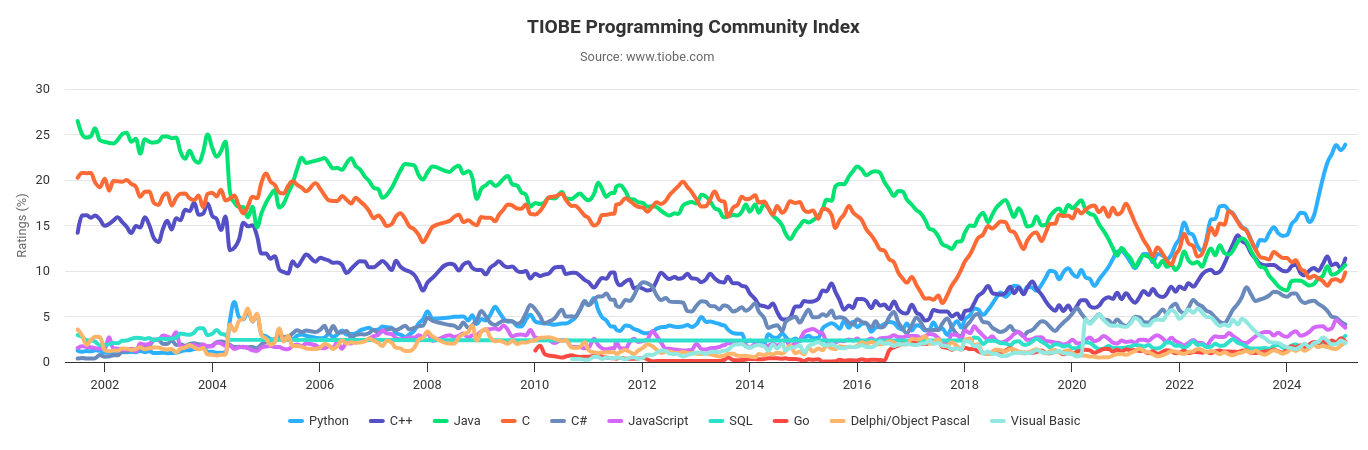
\includegraphics[width=0.8\textwidth]{pictures/Screenshot 2025-02-26 at 19-53-49 TIOBE Index - TIOBE}
        \caption{Entwicklung Tiobe Index 2002 - 2024 vom 26.02.2025 }
        \label{fig:entwicklung-tiobe}
    \end{figure}

    \begin{figure}[h]
        \centering
        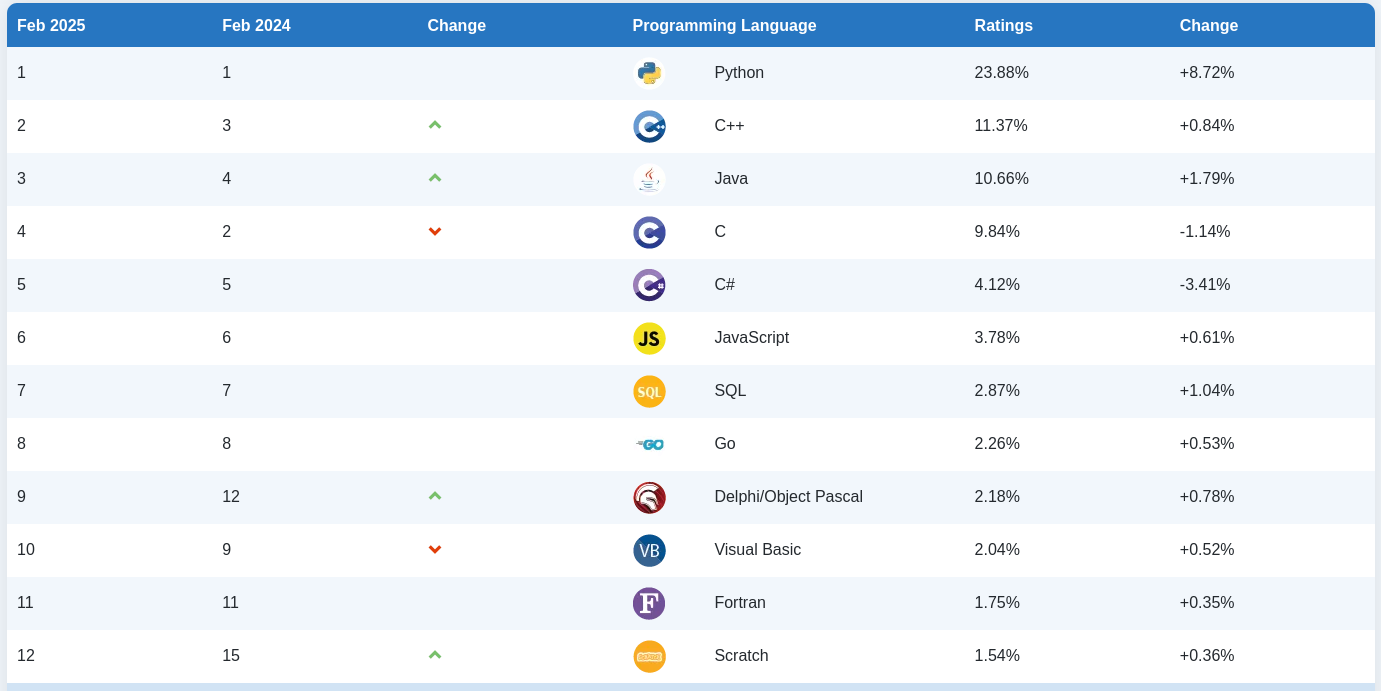
\includegraphics[width=0.8\textwidth]{pictures/Screenshot 2025-02-26 at 19-54-42 TIOBE Index - TIOBE}
        \caption{Tiobe Index Februar 2025 vom 26.02.2025}
        \label{fig:tiobe-java-2025}
    \end{figure}

    \begin{figure}[h]
        \centering
        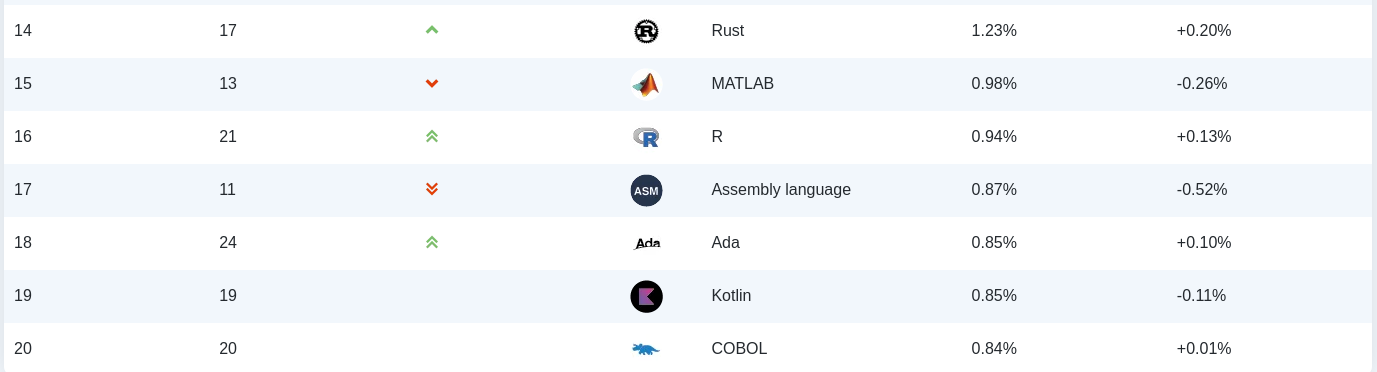
\includegraphics[width=0.8\textwidth]{pictures/Screenshot 2025-03-11 at 22-21-04 TIOBE Index - TIOBE}
        \caption{Tiobe Index März 2025 vom 11.03.2025}
        \label{fig:tiobe-kotlin-2025}
    \end{figure}

    \begin{figure}[h]
        \centering
        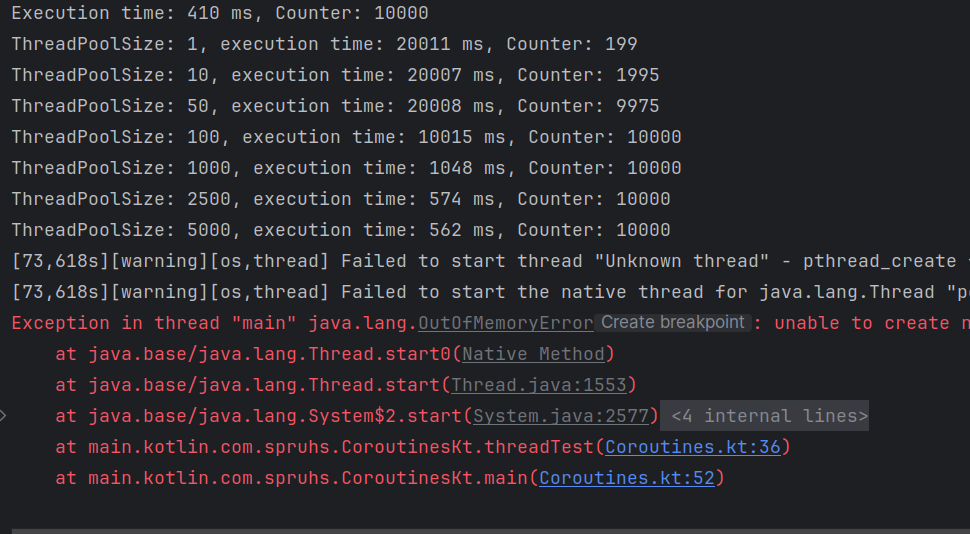
\includegraphics[width=0.8\textwidth]{pictures/Bildschirmfoto vom 2025-04-08 20-09-18}
        \caption{Ausführung Coroutines und Threads}
        \label{fig:coroutines-threads}
    \end{figure}


\end{document}